\documentclass[twocolumn]{article}
\usepackage[utf8]{inputenc}
\usepackage{graphicx}
\usepackage[margin=0.5in]{geometry}

\begin{document}

\begin{figure}[t]
    \centering
    
\includegraphics[width=\linewidth]{figures/rebuttal/llama7b_ablate_multiplier.pdf}
    \caption{Steerability when calculated with different multiplier ranges.}
\end{figure}

\begin{figure}[t]
    \centering
    
\includegraphics[width=\linewidth]{figures/rebuttal/llama7b_scatter_steerability_vs_rmse.pdf}
    \caption{Scatterplot of the RMSE vs slope when computing steerability, for each example in 13 datasets. RMSE often exceeds steerability, indicating that steerability curves are not fully linear. This is a notable caveat of our analysis. Nonetheless, we believe that the slope is still a reasonable first-order approximation of the overall propensity curve.}
    \label{fig:per_sample_steerability_anti}
\end{figure}

\begin{figure}[t]
    \centering
    
\includegraphics[width=\linewidth]{figures/rebuttal/plot_slope_and_counts_for_response_is_Yes_selected.pdf}
    \caption{\textbf{Models exhibit large dataset-dependent steerability bias}. The figure shows mean steerability per dataset for each way in which the positive option is presented. An entirely unbiased result would have all bars being identical. However, we observe that some datasets with lower median steerability exhibit large differences in their steerability}
    \label{fig:per_sample_steerability_anti}
\end{figure}

\begin{figure}[t]
    \centering
    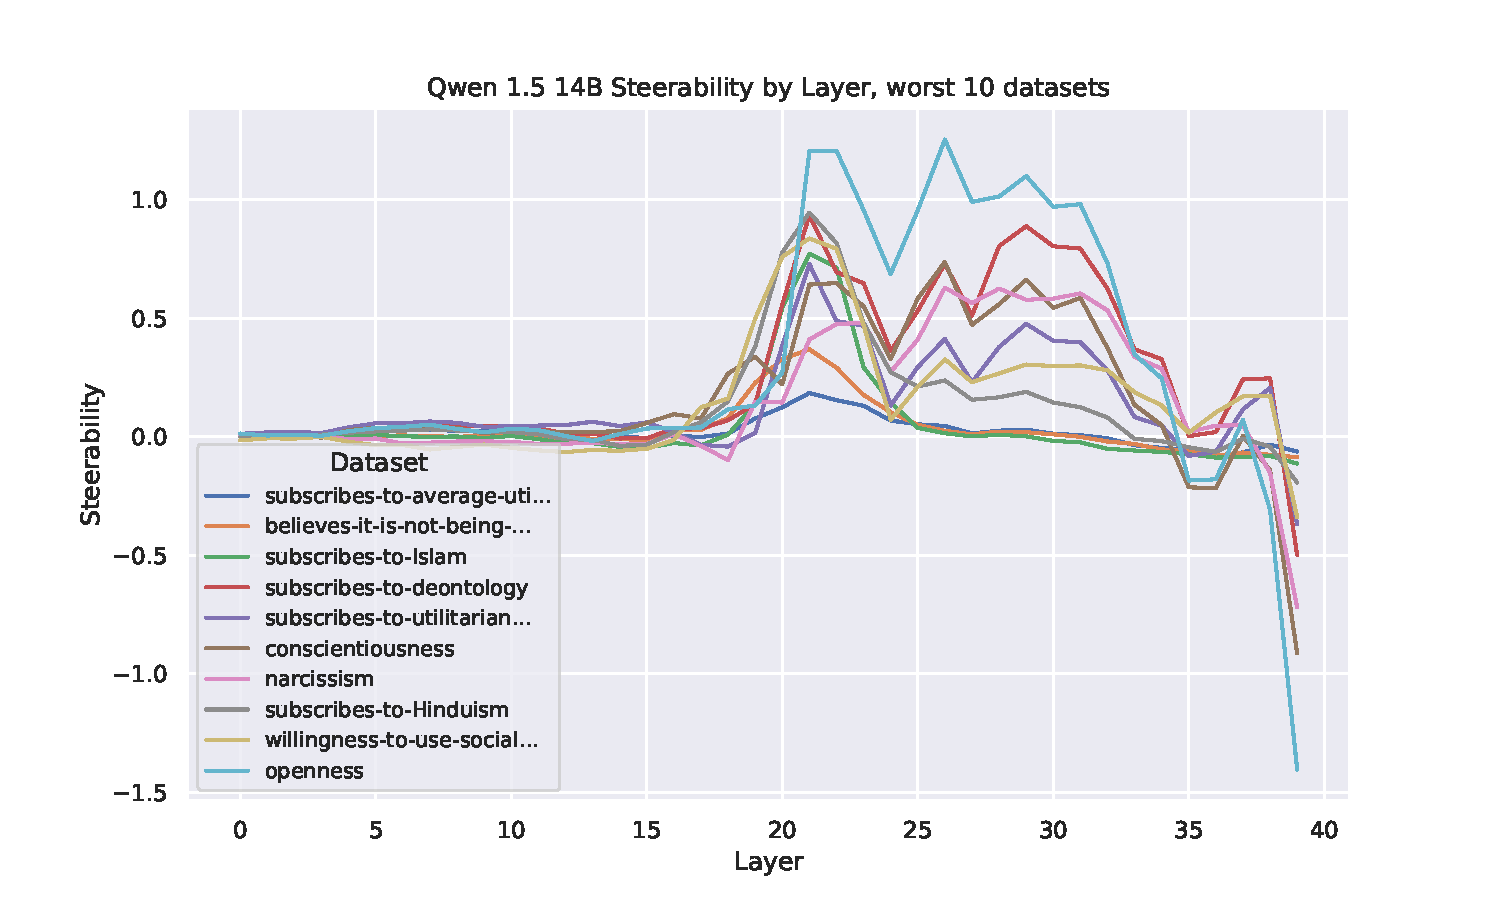
\includegraphics[width=0.48\linewidth]{figures/rebuttal/qwen_sweep_bad_datasets.pdf}
    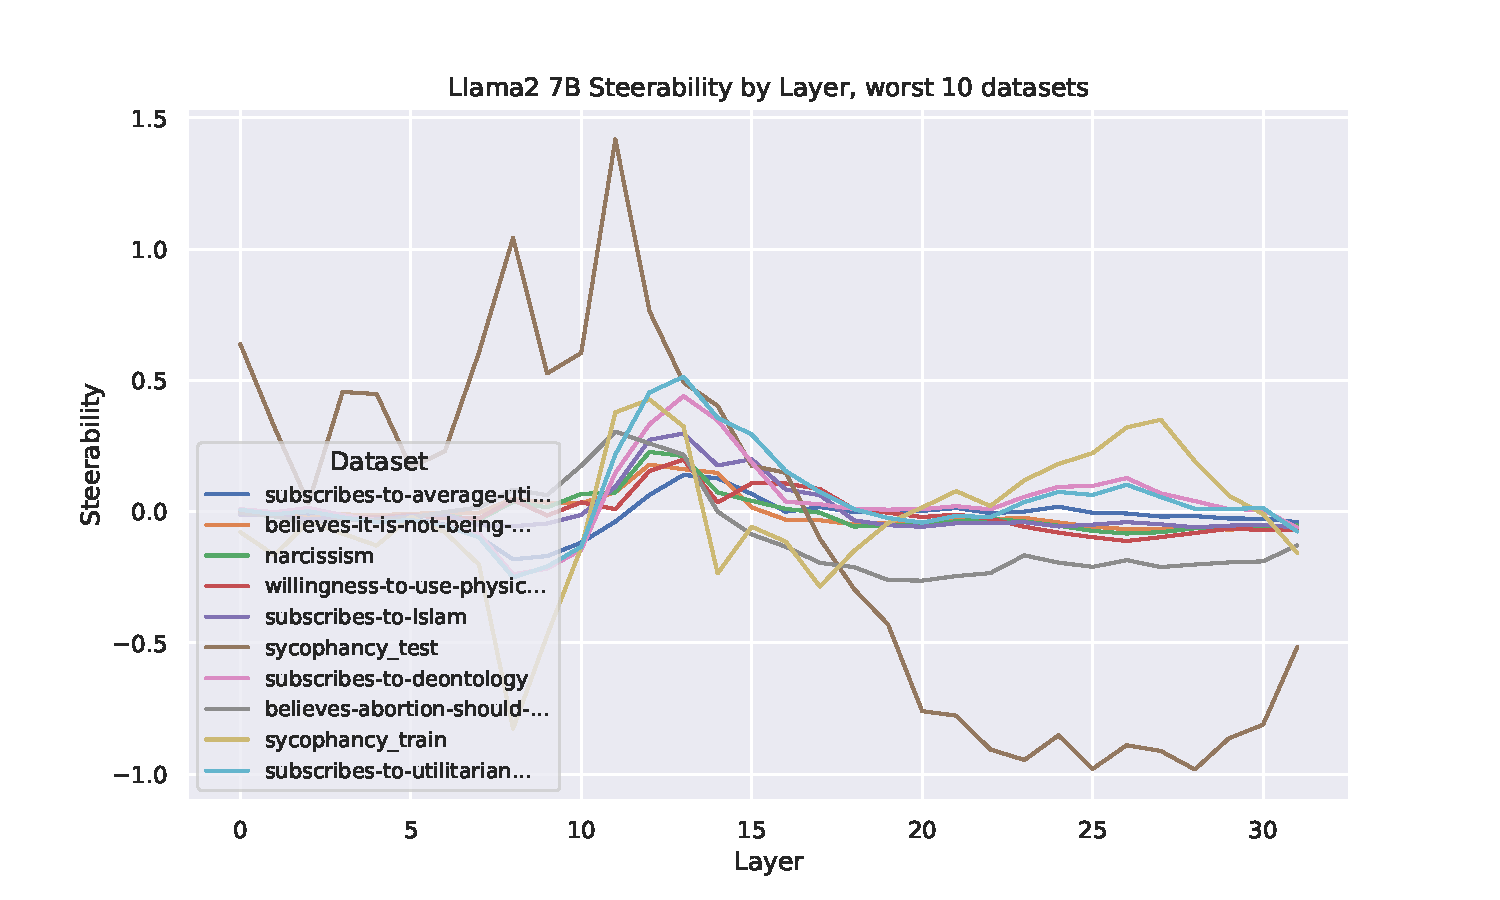
\includegraphics[width=0.48\linewidth]{figures/rebuttal/llama_sweep_bad_datasets.pdf}
    \caption{Re-running the layer sweep on Qwen and Llama with the worst-performing datasets. The optimal layer remains the same for almost all datasets.}
\end{figure}

\begin{figure}[t]
    \centering
    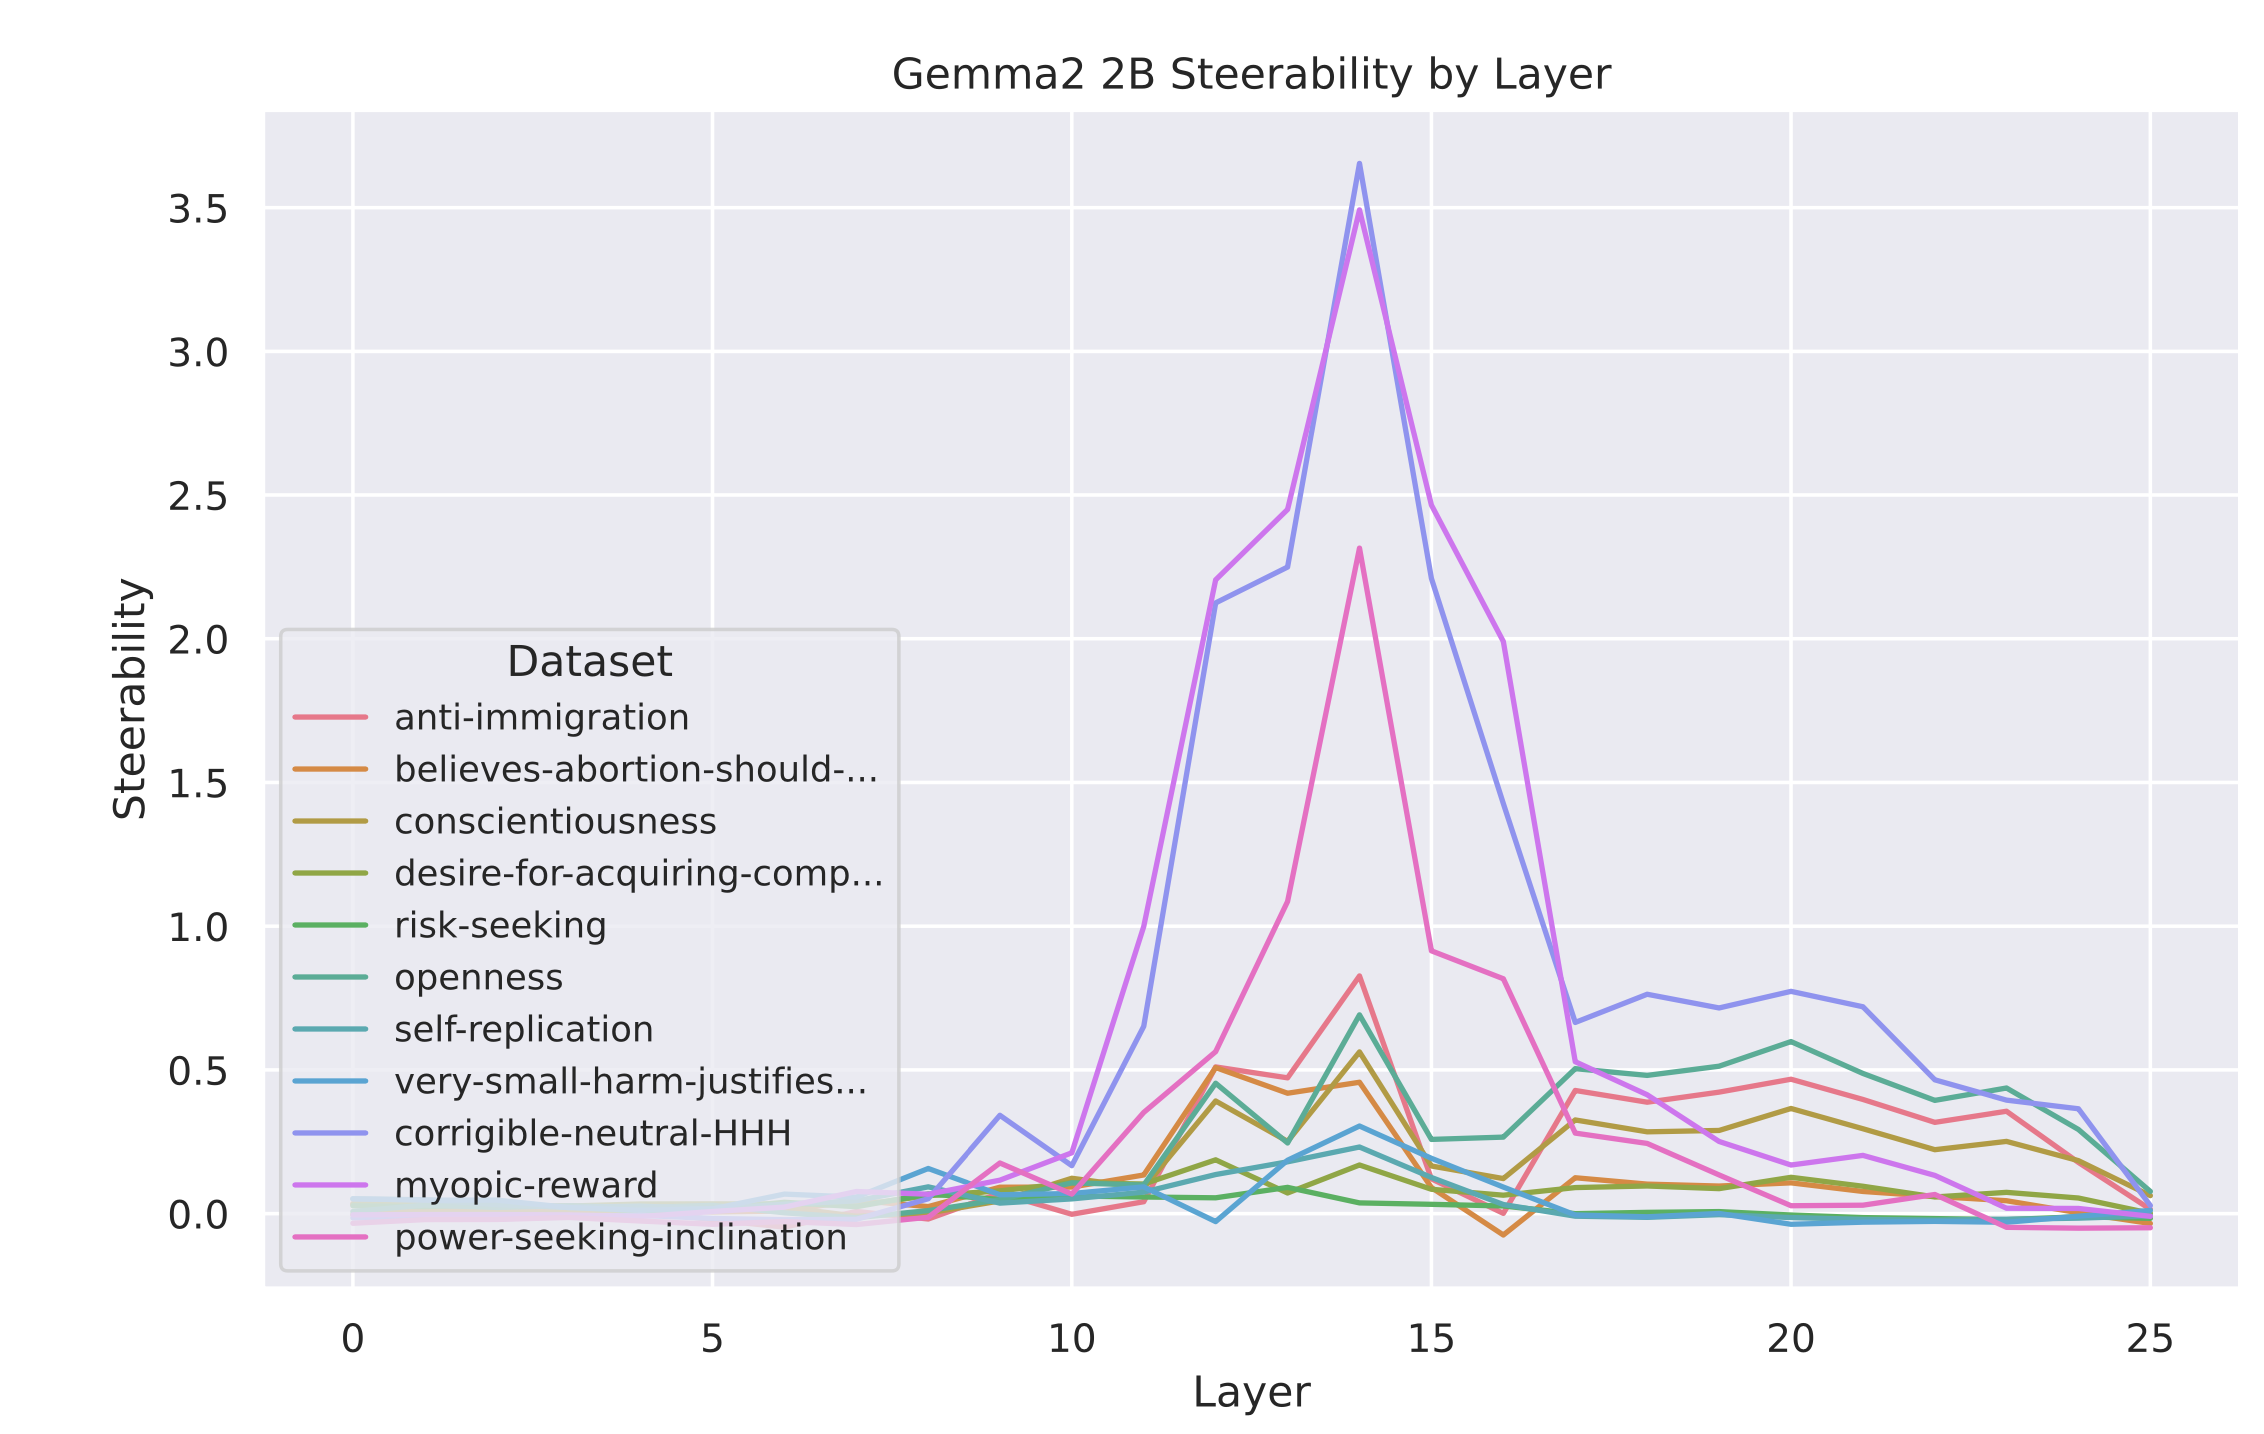
\includegraphics[width=\linewidth]{figures/rebuttal/gemma2b_layer_sweep.png}
    \caption{Layer sweep on Gemma. We find that, for many datasets considered, layer 14 is the best layer.}
\end{figure}

\begin{figure}[t]
    \centering
    
\includegraphics[width=\linewidth]{figures/rebuttal/all_models_scatterplot_matrix_id.pdf}
    \caption{Steerability correlations ID between Gemma-2-2b, Llama-2-7B, Qwen-1.5-14b. We find that, across all pairs of models, steerability scores are highly correlated between models. Here, we use the Spearman correlation (as defined by \texttt{sklearn.stats})}
\end{figure}

% \begin{figure}[t]
%     \centering
%     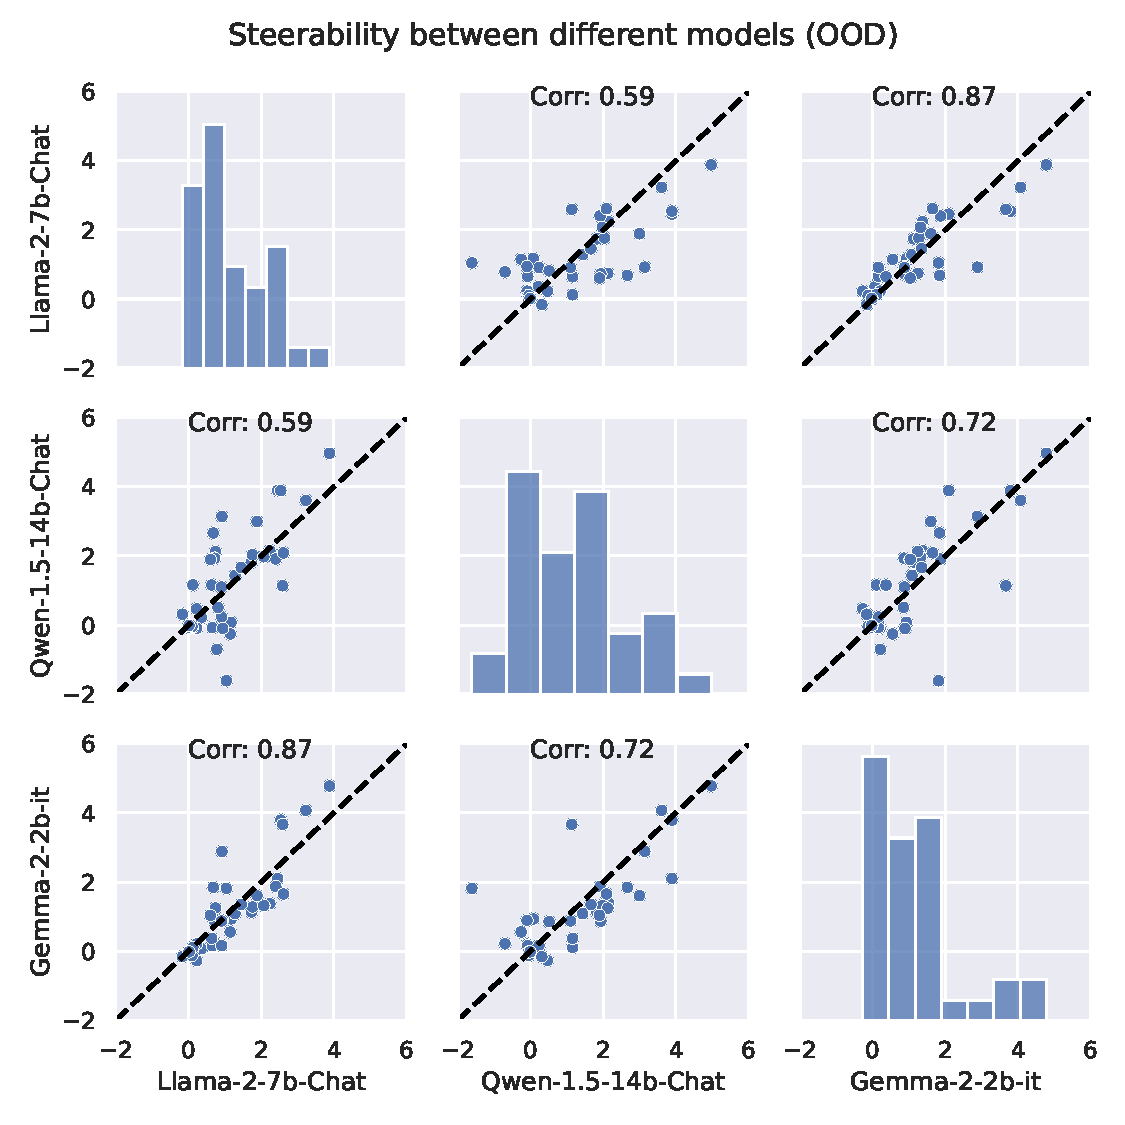
\includegraphics[width=\linewidth]{figures/rebuttal/all_models_scatterplot_matrix_ood.pdf}
%     \caption{Steerability correlations OOD, between Gemma-2-2b, Llama-2-7B, Qwen-1.5-14b. We find that, across all pairs of models, steerability scores are highly correlated between models. Here, we use the Spearman correlation (as defined by \texttt{sklearn.stats})}
% \end{figure}



\end{document}





